\documentclass[11pt]{report} 

\usepackage{projectreport}
\setcounter{tocdepth}{3}
\newcommand{\name}{Eminalp Koyuncu - 2307882}
\newcommand{\course}{EE568 - Selected Topics on Electrical Machines}
\newcommand{\projecttitle}{Project-1: Torque in a Variable Reluctance Machine}
\newcommand{\submissiondate}{April 2026}


% ------------------------------------------------------------------------------
% Document
% ------------------------------------------------------------------------------
\begin{document}

\maketitle

\tableofcontents
% ------------------------------------------------------------------------------
% Top matter
% ------------------------------------------------------------------------------
\section*{Introduction}
\addcontentsline{toc}{section}{Introduction}
\blindtext[1] % creates dummy text
\section*{Analytical Modelling}
\addcontentsline{toc}{section}{Analytical Modelling}

\subsection*{Inductance-Reluctance Calculations}
\addcontentsline{toc}{subsection}{Inductance-Reluctance Calculations}
In this part, we find the minimum reluctance and inductance values of the system analytically. Since we assume that the core is infinitely permeable, the only contribution to the reluctance of the system comes from the air gap. Hence, the maximum reluctance occurs when the air gap cross section is exposed to the maximum air gap length (i.e. 5 mm) uniformly and minimum reluctance occurs when the air gap cross section is exposed to the minimum air gap length (i.e. 1 mm). These two rotor positions are illustrated in Figure \ref{fig:1}.
\begin{figure}[h!]
    \centering
    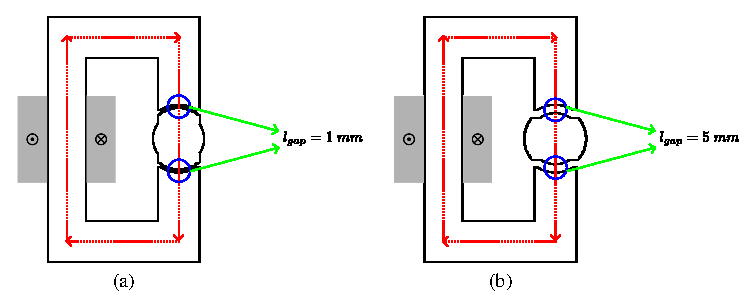
\includegraphics[width=0.9\linewidth]{Images/Fig1_final.eps}
    \caption{Rotor positions for minimum reluctance - maximum inductance and maximum reluctance - minimum inductance configurations and corresponding air gap lengths. (a) shows the minimum reluctance - maximum inductance configuration. (b) shows the maximum reluctance - minimum inductance configuration.}
    \label{fig:1}
\end{figure}

The reluctance contribution of the air gap can be calculated as follows.

\begin{equation}
    \mathcal{R}=\frac{l_{gap}}{\mu_0A_{gap}}
\end{equation}

Assuming that the air gap has a rectangular cross section, we can find the cross section area of the air gap as follows. 

\begin{equation}
    A_{gap} = 15 *25*10^{-6} = 3.75*10^{-4} \; m^2
\end{equation}

So, we can find the maximum and minimum reluctance values as follows.

\begin{equation}
    \mathcal{R}_{min}=\frac{1*10^{-3}}{4\pi*10^{-7}*3.75*10^{-4}}=2.12*10^6 \;At/Wb
\end{equation}

\begin{equation}
    \mathcal{R}_{max}=\frac{5*10^{-3}}{4\pi*10^{-7}*3.75*10^{-4}}=10.6*10^6 \;At/Wb
\end{equation}

We can find the inductance of the system for a given reluctance as follows.

\begin{equation}
    L=\frac{N^2}{\mathcal{R}}
\end{equation}

Where $N$ is the number of turns of the coil. Thus we can find the maximum and minimum inductance values as follows.

\begin{equation}
    L_{max}=\frac{300^2}{\mathcal{R}_{min}}=\frac{300^2}{2.12*10^6} = 42\;mH
\end{equation}

\begin{equation}
    L_{min}=\frac{300^2}{\mathcal{R}_{max}}=\frac{300^2}{10.6*10^6} = 8.5\;mH
\end{equation}

To calculate the variation of inductance as a function of rotor position, we may assume a sinusoidal change in the air gap length as the rotor rotates since the cross section area is not exposed to full minimum or maximum air gap lengths uniformly as the rotor rotates. Let's assume the following air gap length variation as a function of the rotor position, assuming the rotor position is $\theta$ and Figure \ref{fig:1}(a) shows $\theta=0^0$ position. 

\begin{equation}
    l_{gap}(\theta) = 3-2\cos(2\theta) \;mm
\end{equation}

This way, we obtain the minimum air gap length at $\theta=0^0$ and maximum air gap length at $\theta=90^0$. So, the reluctance becomes,

\begin{equation}
    \mathcal{R}(\theta) = \frac{(3-2\cos(2\theta))*10^{-3}}{4\pi*10^{-7}*3.75*10^{-4}}=(6.37-4.24\cos(2\theta))*10^6 \;At/Wb
\end{equation}

Finally, the inductance becomes,

\begin{equation}
    L(\theta)=\frac{300^2}{(6.37-4.24\cos(2\theta))*10^6} \;H = \frac{42.5}{3-2\cos(2\theta)} \;mH
\end{equation}

Plotting the above expression, we get the inductance variation as a function of rotor position given in Figure \ref{fig:2}.

\begin{figure}[h!]
    \centering
    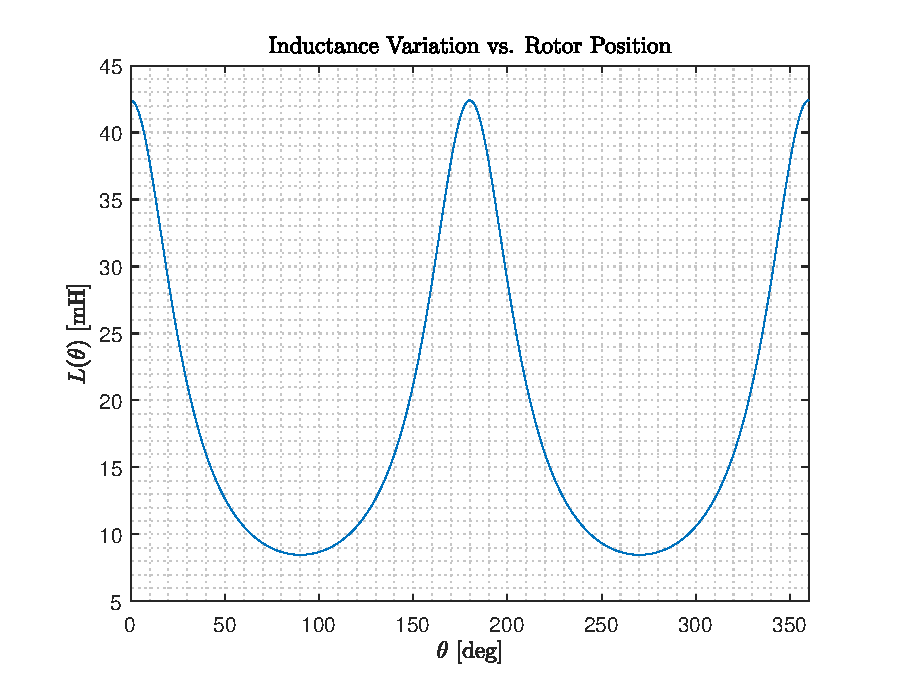
\includegraphics[width=0.9\linewidth]{Images/InductanceVariation.eps}
    \caption{Inductance variation as a function of rotor position.}
    \label{fig:2}
\end{figure}

\subsection*{Torque Calculations}
\addcontentsline{toc}{subsection}{Torque Calculations}

We know that the reluctance torque created by constant excitation can be calculated as follows.

\begin{equation}
    T = \frac{1}{2}I^2\frac{dL(\theta)}{d\theta}
\end{equation}

We can calculate the derivative of the inductance with respect to the rotor angle as follows.

\begin{equation}
    \frac{dL(\theta)}{d\theta}=-\frac{42.5*10^{-3}}{(3-2\cos(2\theta))^2}*4\sin(2\theta)=\frac{170*10^{-3}\sin(2\theta)}{(3-2\cos(2\theta))^2}
\end{equation}

So, the torque expression becomes, 

\begin{equation}
    T=-\frac{2.5^2}{2}\frac{170*10^{-3}\sin(2\theta)}{(3-2\cos(2\theta))^2}=-\frac{0.53}{(3-2\cos(2\theta))^2} \; Nm
\end{equation}

Plotting the torque with respect to the rotor angle, we obtain the response given in Figure \ref{fig:3}.

\begin{figure}[h!]
    \centering
    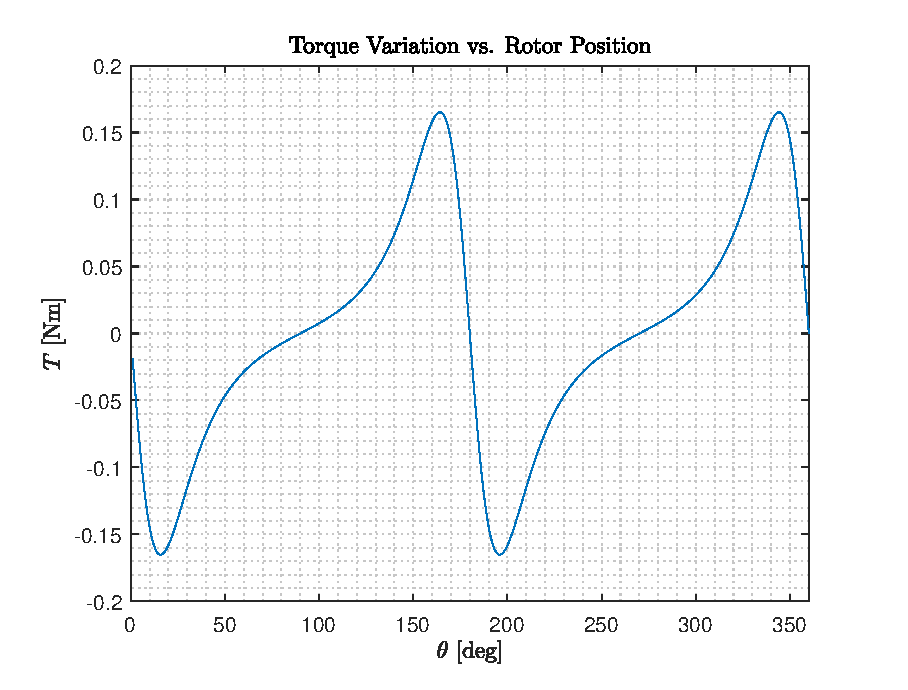
\includegraphics[width=0.9\linewidth]{Images/TorqueVariation.eps}
    \caption{Torque variation as a function of rotor position.}
    \label{fig:3}
\end{figure}


\subsection*{Possible Model Improvements}
\addcontentsline{toc}{subsection}{Possible Model Improvements}

The following model improvements can be made to improve the accuracy of the analytical calculations.

\begin{itemize}
    \item The non-homogeneous flux distribution can be modeled by taking the cross section area smaller than the the original area by some factor.
    \begin{equation}
        A_{eff} = KA_{gap}\;, \qquad K\in [0.5,1]
    \end{equation}
    \item In this part, we assumed that the core is infinitely permeable, which is not the case in a real system and the core has also a contribution to the reluctance. We can also consider this reluctance in the calculations as follows.
    \begin{equation}
        \mathcal{R}_{core} = \frac{l_{core}}{\mu_0\mu_rA_{core}}
    \end{equation}
    \begin{equation}
        \mathcal{R}=\mathcal{R}_{core}+\mathcal{R}_{gap}
    \end{equation}
    \item We can represent the effect of the fringing flux with an increase in the air gap reluctance by some fraction of the theoretical reluctance. If we assume \%10 fringing flux, then,
    \begin{equation}
        \mathcal{R}_{gap,eff}=1.1\mathcal{R}_{gap}
    \end{equation}
    \item For the leakage flux, again, we can represent the effect with an increase in the reluctance of the air gap similar to previous case.
    \item We can also represent the nonlinear behavior of the permeability by taking it as a function of excitation. In this case, the torque expression also depends on the derivative of the excitation current. 
\end{itemize}




\section*{FEA Modelling (2D - Linear Materials)}
\addcontentsline{toc}{section}{FEA Modelling (2D - Linear Materials)}
\blindtext[1] % creates dummy text


\subsection*{Geometry}
\addcontentsline{toc}{subsection}{Geometry}
\subsection*{Meshing}
\addcontentsline{toc}{subsection}{Meshing}
\subsection*{Boundary Conditions}
\addcontentsline{toc}{subsection}{Boundary Conditions}
\subsection*{Solver Settings}
\addcontentsline{toc}{subsection}{Solver Settings}

\subsection*{Results}
\addcontentsline{toc}{subsection}{Results}
\subsubsection*{Flux Density Vectors for $\theta=\{0^0,45^0,90^0\}$}
\addcontentsline{toc}{subsubsection}{Flux Density Vectors for $\theta=\{0^0,45^0,90^0\}$}
\subsubsection*{Inductance and Stored Energy for $\theta=\{0^0,45^0,90^0\}$}
\addcontentsline{toc}{subsubsection}{Inductance and Stored Energy for $\theta=\{0^0,45^0,90^0\}$}
\subsubsection*{Torque Generated in the System}
\addcontentsline{toc}{subsubsection}{Torque Generated in the System}


\section*{FEA Modelling (2D - Nonlinear Materials)}
\addcontentsline{toc}{section}{FEA Modelling (2D - Nonlinear Materials)}
\blindtext[1] % creates dummy text

\subsection*{Results}
\addcontentsline{toc}{subsection}{Results}
\subsubsection*{Flux Density Vectors for $\theta=\{0^0,45^0,90^0\}$}
\addcontentsline{toc}{subsubsection}{Flux Density Vectors for $\theta=\{0^0,45^0,90^0\}$}
\subsubsection*{Inductance and Stored Energy for $\theta=\{0^0,45^0,90^0\}$}
\addcontentsline{toc}{subsubsection}{Inductance and Stored Energy for $\theta=\{0^0,45^0,90^0\}$}
\subsubsection*{Torque Generated in the System}
\addcontentsline{toc}{subsubsection}{Torque Generated in the System}

\section*{Control Method}
\addcontentsline{toc}{section}{Control Method}
\blindtext[1] % creates dummy text

\section*{Conclusion}
\addcontentsline{toc}{section}{Conclusion}
\blindtext[1] % creates dummy text

\addcontentsline{toc}{section}{References}
\renewcommand\bibname{References}
\printbibliography

\end{document}